% Options for packages loaded elsewhere
\PassOptionsToPackage{unicode}{hyperref}
\PassOptionsToPackage{hyphens}{url}
%
\documentclass[
]{article}
\usepackage{lmodern}
\usepackage{amssymb,amsmath}
\usepackage{ifxetex,ifluatex}
\ifnum 0\ifxetex 1\fi\ifluatex 1\fi=0 % if pdftex
  \usepackage[T1]{fontenc}
  \usepackage[utf8]{inputenc}
  \usepackage{textcomp} % provide euro and other symbols
\else % if luatex or xetex
  \usepackage{unicode-math}
  \defaultfontfeatures{Scale=MatchLowercase}
  \defaultfontfeatures[\rmfamily]{Ligatures=TeX,Scale=1}
\fi
% Use upquote if available, for straight quotes in verbatim environments
\IfFileExists{upquote.sty}{\usepackage{upquote}}{}
\IfFileExists{microtype.sty}{% use microtype if available
  \usepackage[]{microtype}
  \UseMicrotypeSet[protrusion]{basicmath} % disable protrusion for tt fonts
}{}
\makeatletter
\@ifundefined{KOMAClassName}{% if non-KOMA class
  \IfFileExists{parskip.sty}{%
    \usepackage{parskip}
  }{% else
    \setlength{\parindent}{0pt}
    \setlength{\parskip}{6pt plus 2pt minus 1pt}}
}{% if KOMA class
  \KOMAoptions{parskip=half}}
\makeatother
\usepackage{xcolor}
\IfFileExists{xurl.sty}{\usepackage{xurl}}{} % add URL line breaks if available
\IfFileExists{bookmark.sty}{\usepackage{bookmark}}{\usepackage{hyperref}}
\hypersetup{
  hidelinks,
  pdfcreator={LaTeX via pandoc}}
\urlstyle{same} % disable monospaced font for URLs
\usepackage{longtable,booktabs}
% Correct order of tables after \paragraph or \subparagraph
\usepackage{etoolbox}
\makeatletter
\patchcmd\longtable{\par}{\if@noskipsec\mbox{}\fi\par}{}{}
\makeatother
% Allow footnotes in longtable head/foot
\IfFileExists{footnotehyper.sty}{\usepackage{footnotehyper}}{\usepackage{footnote}}
\makesavenoteenv{longtable}
\usepackage{graphicx}
\makeatletter
\def\maxwidth{\ifdim\Gin@nat@width>\linewidth\linewidth\else\Gin@nat@width\fi}
\def\maxheight{\ifdim\Gin@nat@height>\textheight\textheight\else\Gin@nat@height\fi}
\makeatother
% Scale images if necessary, so that they will not overflow the page
% margins by default, and it is still possible to overwrite the defaults
% using explicit options in \includegraphics[width, height, ...]{}
\setkeys{Gin}{width=\maxwidth,height=\maxheight,keepaspectratio}
% Set default figure placement to htbp
\makeatletter
\def\fps@figure{htbp}
\makeatother
\setlength{\emergencystretch}{3em} % prevent overfull lines
\providecommand{\tightlist}{%
  \setlength{\itemsep}{0pt}\setlength{\parskip}{0pt}}
\setcounter{secnumdepth}{-\maxdimen} % remove section numbering

\usepackage{tabularx}
\usepackage{graphicx}
\usepackage{booktabs}
\usepackage{caption}
\usepackage{geometry}

\author{}
\date{}

\begin{document}

\hypertarget{abstract}{%
  \section{Abstract}\label{abstract}}

Electric load peak shaving is a challenging and important problem
considering the rapid growth of high power electric vehicle charging
sites. Co-located solar photovoltaic provides locally produced energy,
but an additional storage battery is required for reliable peak shaving.
With occasional evening load peaks and an electric tariff with a
16:00-21:00 peak time of use period, vertical bifacial modules facing
West have an economic advantage due to more of the production shifted
into the late afternoon and early evening. Exploiting this, an optimal
electric load peak shaving simulator dispatches a stationary battery to
minimize the retail electric cost incurred by a real electric vehicle
charging site over 10 months. Five different case studies of co-located
bifacial solar photovoltaic arrays are simulated, a base case oriented
South and tilted at 20° and four experimental cases where a percentage
(25\%, 50\%, 75\%, or 100\%) of the array is oriented West and tilted at
90°. The problem is formulated such that the optimizer minimizes the
retail electric cost by adjusting three peak power thresholds, each
corresponding to a time of use period with an associated power price in
\(\$/kW\). The optimizer is implemented using a Newton-Raphson gradient
descent approach and the optimality of the method is verified to within
0.1 \(kW\). A sensitivity analysis on battery energy capacity results in
a largest cost reduction, relative to the South 20° base case, of \$1422
(6.7\%) achieved by the 50\% West 90° case and a modest 25 kWh battery.
A second sensitivity analysis on solar power capacity shows that the
cost reduction increases monotonically and logarithmically for all cases
and battery capacities. The largest cost decrease is \$2579 (16.1\%),
achieved by the 75\% West 90° case at 200\% of nominal solar capacity
along with a 125 kWh battery. Both data and code are shared to the
public on GitHub.

\hypertarget{introduction}{%
  \section{Introduction}\label{introduction}}

\hypertarget{why-peak-load}{%
  \subsection{Why peak load}\label{why-peak-load}}

The renewable energy transition will oversee a global shift toward
electric energy consumption and renewable electric energy production in
the coming decades. Since most electric transmission and distribution
networks were previously built slowly over the span of many decades,
electric load growth will almost definitely outpace network upgrades.
And where these upgrades are completed they are necessarily an
additional cost paid by all electricity consumers, due to the decrease
in the load factor. Furthermore in some markets where companies can own
both generation and distribution, business-as-usual infrastructure
upgrades may be prioritized over the new construction of more complex
and financially risky renewable generators. So while there are some
creative solutions around dynamic capacity limits, two important
solution areas for overall deployment speed, cost effectiveness, and
overall decarbonization goals are (a) more local energy production and
(b) increasing the load factor.

Electric vehicle (EV) charging and electric heating and cooling,
including traditional air conditioning and heat pumps, are two common
new loads that will strain networks in most countries. Heat pump and air
conditioning load factor may be increased with architectural features
such as insulation and thermal storage, but building retrofits are often
slowed down due to permitting and other challenges. Meanwhile extreme
weather events, especially heat waves, will likely further reduce the
load factor of these devices. Many EV users will choose to slowly charge
overnight at home for convenience and to minimize their energy cost.
However workplace, fleet, and public EV charging stations will likely
still be required, and these may especially suffer from a low load
factor due to the convenience or need of fast charging at high power.

\hypertarget{peak-shaving}{%
  \subsection{Peak shaving}\label{peak-shaving}}

Peak load management, or peak shaving, essentially requires choosing a
power threshold and holding the load power below it. Controllable loads,
energy storage, or generation assets behind the billing meter can all be
used to reduce the load power to the threshold power. The threshold may
only apply for only certain time periods. There may be multiple
thresholds and periods each day, month, or year. There are two general
cases of peak shaving worth considering. The most generation formulation
of peak shaving control is formulated in Equation \ref{eg:peakshaving-general}.

\begin{equation}
  \label{eg:peakshaving-general}
  \begin{split}
    I_{threshold,t} &> I_{j,t} - \Sigma_i I_{gen,i,t} - \Sigma_j I_{gen,up,j,t} - \Sigma_k I_{load,dn,k,t}  \\
    \\
    &\text{where:} \\
    &i\text{ is generation asset with no flexibility} \\
    &j\text{ is generation asset with upward flexibility} \\
    &k\text{ is controllable load asset with downward flexibility} \\
    &t\text{ is relevant timesteps}
  \end{split}
\end{equation}

Here we consider the case of no controllable load, a single battery,
solar which reduces the site load, and all values in units of average
real power over the interval \(\Delta h = 1\ hour\). This is descrbied in Equation \ref{eq:peakshaving}.

\begin{equation}
  \label{eq:peakshaving}
  \begin{split}
    P_{threshold,h} &> P_{load,h} - P_{solar,h} - P_{batt,discharge,h} + P_{batt,charge,h}   \\
    &\text{where:} \\
    P_{batt,discharge,h} &\ge 0 \\
    P_{batt,charge,h} &\le 0 \\
    h &\in \{0,1,2,...23\} \\
  \end{split}
\end{equation}

\hypertarget{technical}{%
  \subsubsection{Technical}\label{technical}}

Technical peak shaving refers to the case where a load must operate
under a technical limitation such as a maximum power agreement or
distribution transformer size. The load power must remain under the
threshold at all times, otherwise there may be a technical failure such
an activated overcurrent protection. Even if the load is technically
able to rise above the threshold, doing so may violate a contract
regarding maximum load power. The important consideration is that the
economic cost of failure to hold the load under the threshold is
prohibitively high. The time resolution of technical peak shaving
control and modeling may need to be as low as seconds or milliseconds.
Although this may be a challenging problem if the current limit is
dynamically set or if a larger network is considered, from the
perspective of dispatching the assets to shave the peak the problem is a
relatively simple one: economic dispatch such that the the load current
remains below the threshold current. Technical peak shaving might be
performed on current or apparent power rather than active power.

\hypertarget{economic}{%
  \subsubsection{Economic}\label{economic}}

Rather, economic peak shaving aims to reduce what a consumer pays for
power and possibly also energy. Medium and large electric consumers
often pay a price on energy (€\(/kWh\)) and a price on power
(€\(/kWh_{peak}\)), also called a demand charge. The energy cost
(€\(/kWh \times E_{consumed}\)) may vary with time of day, day of week,
and season of the year, which is often referred to as time of use or
peak pricing. Where there is a sufficient spread between the peak and
off-peak prices there may be the opportunity to curtail load during high
prices, use controllable loads to shift from a high price period to a
lower one, or to use energy storage to buy energy at the lower price and
reduce load during a higher price period. A peak shaving approach
applied to the energy cost could be effective and maybe even
advantageous. However there are several key differences between an
energy based approach and a power one, where peak shaving is better
suited for the latter.

Instead, the power cost (€\(/kW \times P_{max}\) ) typically applies to
the max power during the billing period, where the peak power is the
maximum non-moving average in a given period (e.g. 12:00-18:00 on
weekdays) calculated on a given interval (e.g. 60 minutes). Similar to
the energy cost, there may be multiple time of use periods and
associated prices, such as peak, mid-peak, and off-peak. And where the
spread price is sufficiently high, the period peak can be reduced with
load curtailment or rescheduling, distributed generation such as solar,
or energy storage.



\begin{table}
    \centering
    \caption{Economic and Technical Peak Shaving Comparison}
    \label{tab:econ-tech-peak-shaving}
    \begin{tabularx}{\textwidth}{XXX}
    \toprule
    Feature & Technical Peak Shaving & Economic Peak Shaving  \\
    \midrule
    Consequence of exceeding the threshold & Damage to infrastructure,possible outage & Monetary cost depending on tariff \\
    Averaging interval                     & 1 minute                                 & 15 minutes or 1 hour (typical) \\
    Valid times of day                     & All                                      & Limited (e.g. 16:00 to 21:00) \\
    Peak is reset every..                  & Never                                    & Month, year, day (typical) \\
    \bottomrule
    \end{tabularx}
\end{table}


\hypertarget{methodology}{%
  \section{Methodology}\label{methodology}}

\begin{figure}
  \centering
  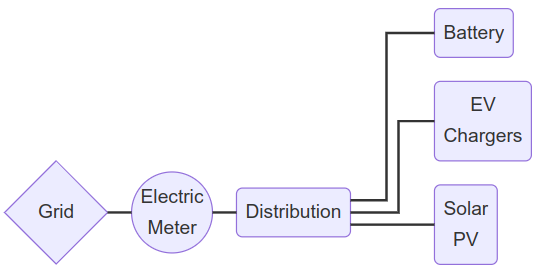
\includegraphics[width=5cm,height=\textheight]{./images/oneline.png}
  \caption{Charging Site One Line Schematic. Simplified
  one-line schematic of the simulated EV charging station with true
  measured EV charging power, modelled on-site solar generation, and a
  modelled stationary battery for economic peak shaving.}
  \label{fig:oneline}
\end{figure}

The methodology of this study is a set of offline simulations involving
(a) EV charging power measurements, (b) modelled solar photovoltaic (PV)
production power, and (b) AC-coupled battery dispatch, all behind the
retail electric meter. These are represented in in Figure \ref{fig:oneline}.
In each simulation the battery power is chosen
such that the net load (natural load less solar production, Equation \ref{eq:net-load}) is held
below a given threshold, which is optimally chosen by a gradient descent
optimizer.

\begin{equation}
  \label{eq:net-load}
  \begin{split}
    NL &= L - S \\
    &\text{where:} \\
    &L(t) \text{ is EV charging load time series (non-negative)}\ [kW]\\
    &S(t) \text{ is solar production time series}\ [kW] \\
  \end{split}
\end{equation}

The optimal threshold changes for each time of use (TOU)
period. A single simulation is defined for one solar configuration and
battery capacity and lasts one calendar month, which is the shortest
period for which the cost function is defined. Simulations are repeated
for several months of data, and many different solar and battery design
sizes, allowing for a retail energy cost comparison among different
design scenarios. EV charging power or solar are never curtailed. The
primary decision variables in each time step are (a) battery charge or
discharge, and (b) battery power.

\hypertarget{data}{%
  \subsection{Data}\label{data}}

\hypertarget{ev-charging-load}{%
  \subsubsection{\texorpdfstring{EV Charging Load
    }{EV Charging Load }}\label{ev-charging-load}}

The measured EV charging power ("load") is from the Caltech Adaptive
Charging Network database at the Jet Propulsion Lab (JPL) site. Each
charging session provides time series active power, averaged over a 10
second interval. In the cases when complete time series data is not
available for a session, the charging profile is estimated and the total
charging energy delivered is the same. The disaggregated session time
series data is summed into a single time series of total site charging
power, which is then averaged over 15-minute intervals. Time stamp
indices refer to the beginning of the 15-minute interval. The data
period is from 2018-5-1 00:00 to 2019-2-28 23:45.

\hypertarget{solar-production}{%
  \subsubsection{Solar Production}\label{solar-production}}

The modelled PV production power begins life as Geostationary
Operational Environmental Satellite (GOES) satellite solar irradiance
data from the US National Solar Resource Database (NSRDB), and is
specific to the exact time and date rather as opposed to typical
meteorological year data. See Table \ref{tab:data-summary}. Prism Solar 350 W bifacial solar module DC
electrical power is estimated using the California Energy Commission
Performance Model, a 6-parameter physical PV cell model. The full AC
array power is estimated given loss assumptions and an inverter
efficiency lookup table in the US National Renewable Energy Laboratory
(NREL) System Advisor Model (SAM) database for the Enphase IQH 380 W
microinverter. All these functions are implemented in SAM v2022.11.21.

Five different solar array orientations are modelled and simulated in
different case studies. See Table \ref{tab:casestudies}. Each orientation has the same number and type of bifacial
modules. In the first orienation all modules facing South at 20° tilt. In the remaining four
orientation a percentage of the modules face all modules face West at 90° tilt: 25\%, 50\%, 75\%, and then 100\%.
Tilt is defined as 90° minus the altitude angle of the normal vector of the primary active face of 
the module. No shading is considered. Of the two sides of the bi-facial module, the primary active 
face is oriented West since afternoon load is generally subject to higher prices.

\begin{table}[!h]
  \centering
  \caption{Timeseries Data Summary. EV charging power is
  measured every 10 seconds for 10 months at the Jet Propulsion
  Laboratory, CA, USA. Solar irradiance from the GOES satellite is
  acquired for the same location. Solar PV array production is modelled
  from the satellite irradiance using a 6 parameter PV cell model and
  inverter efficiency lookup table.\label{tab:loadsectors}}
  \label{tab:data-summary}
  \begin{tabularx}{\textwidth}{XXXXX}
  \toprule
  Timeseries Description & Location & Type & Interval / Length & Source  \\
  \midrule
  \vtop{\hbox{\strut EV charging power}\hbox{\strut (\(kW_{ac}\))}} & Jet
  Propulsion Lab, Pasadena CA, USA                                  & Measured and aggregated from multiple
  EV chargers at single site                                        & 10 sec (average downsampled to 15 min) / 10
  months                                                            & Caltech ACN \\

  \vtop{\hbox{\strut Solar irradiance }\hbox{\strut (\(W/m^2\))}}   & GPS:
  34.2013, -118.1721 (2x2 km square)                                & GOES satellite irradiance                                 & 5
  minute / 10 months                                                & NSRDB PSMv3 \\

  PV array production (\(kW_{ac}\))                                 & GPS: 34.2013, -118.1721 (2x2 km
  square)                                                           & Modelled from satellite irradiance, 368 Prism Solar 350 W
  bifacial modules, 368 Enphase IQH 380 W microinverters            & 15 minute / 10
  months                                                            & SAM (Gilman 2015) \\

  \bottomrule
  \end{tabularx}
\end{table}

\hypertarget{battery}{%
  \subsection{Battery}\label{battery}}

A stationary, storage battery system is simulated as the primary
decision variable in the peak shaving algorithm. In each timestep the
battery is chosen to charge or discharge within its technical limits.
Because the control action is to hold the power exchange with the grid
to below a certain threshold, batteries with a larger power capacity or
energy capacity will necessarily achieve a lower threshold if the entire
battery capacity is used. For a given energy capacity (\(kWh\)) those
limits are a charge or discharge rate no more than 1C and state of
charge (SOC) between 0 and 100\% of rate. State of energy (SOE) is the
SOC multiplied by nominal energy capacity and is used in plots because
the units are more meaningful when comparing dispatch time series.
Half-round-trip charge and discharge efficiency is constant at 90\% and
no self discharge or thermal limiting are considered.

There are many strategies for optimal battery sizing, but the emphasis
in this work is instead on understanding the dynamics between load,
shape of the solar curve, and peak shaving algorithm for a given battery
size. Therefore a sensitivity analysis is performed on the battery
energy capacity, but no one battery size is declared economically
optimal.

Each simulation assumed charge and discharge rate are limited to 1C,
usable SOC is assumed 100\%, and self discharge, parasitic losses, and
thermal limiting are not considered.

\hypertarget{electric-tariff}{%
  \subsection{Electric Tariff}\label{electric-tariff}}

A typical California electric tariff is applied at the point of the
retail electric meter with several different TOU periods and prices. See Table \ref{tab:tariff}.
For the chosen tariff each TOU period may have an energy price
(\(\$/kWh\)), a power price (\(\$/kW\)), or both. The prices may also
change between seasons, and have long term trends like any retail
electric prices. Here a price on power ("demand charge") is understood
as a \(\$/kW\) price applied to the monthly maximum power observed at
the meter, calculated as the 15-minute average of real power.

\begin{table}[!h]
  \centering
  \caption{Retail Electric Tariff. An applicable electric
  tariff schedule with seven different TOU periods for energy and power
  prices, varying by hours of the day and season of the year. From
  California PG\&E.}
  \label{tab:tariff}
  \begin{tabularx}{\textwidth}{XXXXX}
  \toprule
  Name                                   & TOU Period                                               & Summer (Jun 1 - Sept 30) {[}\${]}                   & Winter (Oct 1 -Feb 28) {[}\${]}   & Spring (Mar 1 - May 30) {[}\${]}  \\
  \midrule
  All hours                              & 0:00-0:00                                                & 26.07 / kW                                          & 26.07 / kW      & 26.07 / kW \\
  Super off-peak                         & 9:00-14:00                                               & -\/-                                                & -\/-            & 0.079 / kWh \\
  Off-peak spring                        & \vtop{\hbox{\strut 0:00-9:00,14:00-16:00,}\hbox{\strut 21:00-0:00}} & -\/-                                                     & -\/-              & 0.132 / kWh \\
  Off-peak winter                        & 0:00-16:00, 21:00-0:00                                   & -\/-                                                & 0.132 / kWh     & -\/-\\
  Off-peak summer                        & 0:00-14:00, 23:00-0:00                                   & 0.132 / kWh                                         & -\/-            & -\/-\\
  Partial-peak                           & 14:00-16:00, 21:00-23:00                                 & \vtop{\hbox{\strut 6.81 /
  kW,}\hbox{\strut 0.159 / kWh}}         & -\/-                                                     & -\/-\\
  Peak                                   & 16:00-21:00                                              & \vtop{\hbox{\strut 32.90 / kW,}\hbox{\strut 0.196 /
  kWh}}                                  & \vtop{\hbox{\strut 2.22 / kW,}\hbox{\strut 0.172 / kWh}} & \vtop{\hbox{\strut 2.22 / kW}\hbox{\strut ,0.172 / kWh}}\\
  
  Consequence of exceeding the threshold & Damage to infrastructure,possible outage & Monetary cost depending on tariff \\
  \bottomrule
  \end{tabularx}
\end{table}

The total retail electric cost \(C\) for each month is then the sum of
the energy cost and power cost for the month, where the energy and power
costs are calculated separately for each TOU period. See Equation \ref{eq:cost}. The energy cost is
the energy delivered to the site multiplied by the energy price for that
TOU period. The power cost is the maximum 15-minute average power for
the month multiplied by the power price for that TOU period. Only
positive values of site load \(SL\) are used in the cost calculation
since the monthly peak power for each TOU period must always be positive
and necessarily cannot benefit from net metering (export to the grid).

\begin{equation}
  \label{eq:cost}
  \begin{split}
    C_m &= \Sigma_k^K [ p_{p,k,m} max(NL^+_{k,m} + B_d - B_c + p_{e,k,m} \Sigma (NL^+_{k,m} + B_d(t) - B_c(t)) ] \\
    \\
    & \text{where:} \\
    & NL^+(t) = NL(t),\ \forall\ NL(t)>0\\
    &B_c(t) \text{ is battery charging power time series(non-negative)}\ [kW]\\
    &B_d(t) \text{ is battery discharging power time series(non-negative)}\ [kW] \\
    &C_m \text{ is total retail electric cost for month}\ m\ [\$] \\
    &p_{p,k,m} \text{ is power price for TOU period}\ k\ \text{and month}\ m\  [\$/kW] \\
    &p_{e,k,m} \text{ is energy price for TOU period}\ k\ \text{and month}\ m\ [\$/kWh] \\
    &K \text{ is number of TOU periods}
  \end{split}
\end{equation}

\hypertarget{peak-shaving-algorithm}{%
  \subsection{Peak Shaving Algorithm}\label{peak-shaving-algorithm}}

An optimal peak shaving strategy is used to minimized the total retail
electric cost to the EV charging station. The strategy is operational
only, and assumes the solar production timeseries and battery capacity
are fixed. The state variable controlled by the algorithm is battery
charge or discharge power. However the algorithm reframes the problem as
one of choosing a power threshold \(T\ (kW)\) applied to the point of
injection to the grid, the electric meter. The battery is then
dispatched, within its technical limits, to hold the net load (natural
load less solar production) below the threshold. When the algorithm is
successful the different thresholds for each TOU period are met for an
entire month. If the battery reaches a technical limit and net load
exceeds a threshold, the simulation is not necessarily invalid but is
not likely to minimize the retail electric cost to the site for that
combination of solar and battery size. The peak shaving logic is
described in Figure \ref{fig:peakshaving-flowchart}.

\begin{figure}
  \centering
  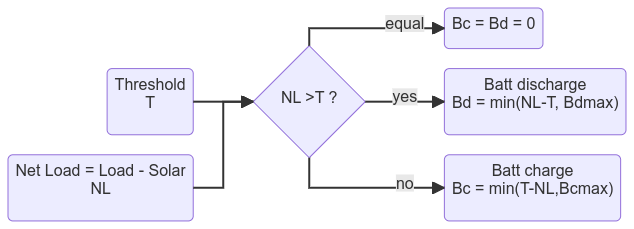
\includegraphics[width=10cm,height=\textheight]{./images/peak shaving flowchart.png}
  \caption{Peak Shaving Flowchart. Net load is the
  timeseries of load less solar. There is one threshold value for one for
  each TOU period with a non-zero power price. For each timestep of the
  simulation the net load is compared to the threshold of that TOU period,
  and the battery is discharged if the net load is greater than the
  threshold and charged if the net load is less than the threshold. If the
  two are equal the battery does nothing. For timesteps with no price on
  power the the battery does nothing.}
  \label{fig:peakshaving-flowchart}
\end{figure}

The peak shaving algorithm describes stepping through time and
dispatching the battery according to power thresholds, but not how the
thresholds are chosen.

\hypertarget{threshold-optimizer}{%
  \subsection{Threshold Optimizer}\label{threshold-optimizer}}

The optimal demand thresholds (one per TOU period) are determined by a
custom gradient descent optimizer. The objective function \(C\)
minimizes the retail energy cost of one month, which is the billing
interval of this retail electric tariff. See Equation \ref{eq:optimization}. In practice the optimal
thresholds are different for each month. The threshold for each TOU
period \(T_k\) is not enforced to be non-negative, but in practice is
always is because the cost function \(C_m()\) cannot evaluate to a
negative value.

\begin{equation}
  \label{eq:optimization}
  \begin{split}
    min[C_m(B_c,B_d)] & = min[C_m(T_1,T_2,..T_K)] \\
    & s.t. \\
    B_c(t) & \le B_{c,max} \\
    B_d(t) & \le B_{d,max} \\
    SOC_{min} & \le SOC \le SOC_{max} \\
    \\
    & \text{where:} \\
    T_k & \text{ is threshold for}\ k\text{-th TOU period of}\ K\ \text{total periods} \\
    SOC(t) & \text{ is battery state of charge timeseries}\ [\frac{kWh}{kWh}] \\
  \end{split}
\end{equation}

Beginning from an initial guess the Newton-Raphson gradient descent
optimizer calculates the batch gradient and updates parameters based on
a learning rate of 0.01. This continues until the stopping condition is
met, minimum cost for a patience of 50 iterations. The Newton-Raphson
gradient descent based optimization method is preferred over linear
programming because it will minimize over a variety of cost functions
without needing to reformulate the linear program.

\hypertarget{simulations}{%
  \subsection{Simulations}\label{simulations}}

Simulations are run one month at a time for a given solar array
orientation and battery capacity, according to the flowchart in Figure \ref{fig:simulation-flowchart}.
The computational environment is Python 3.8 in Windows 10 64-bit, on
an Intel i9 CPU with 64 GB of RAM.

\begin{figure}
  \centering
  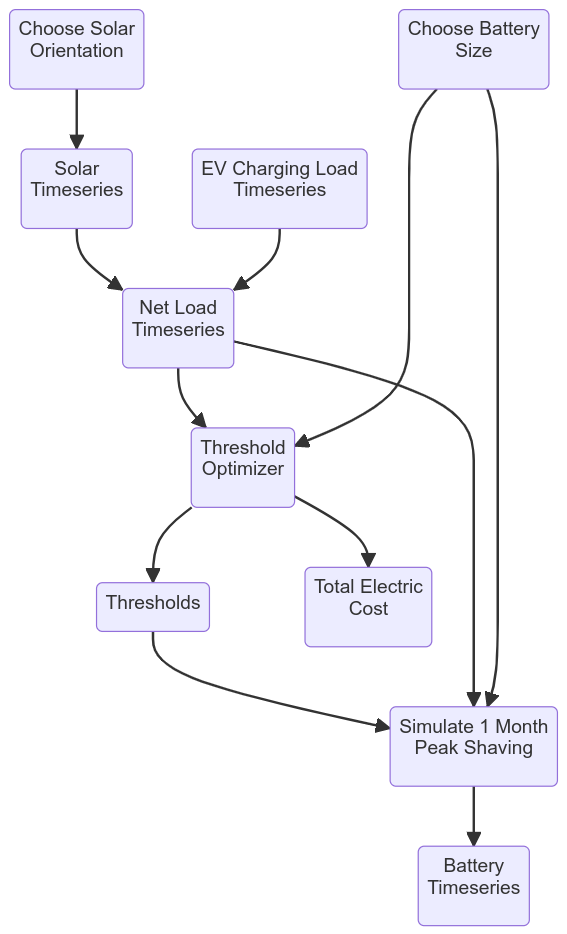
\includegraphics[width=15cm,height=\textheight]{./images/simulation flowchart.png}
  \caption{Simulation Flowchart. Given a solar orientation
  and chosen battery capacity, the net load timeseries is calculated from
  EV charging load and solar production. The threshold optimizer produces
  one threshold value (kW) for each TOU period with non-zero power prices.
  This returns both optimal thresholds and a minimum cost. Lastly a 1
  month simulation of the battery charging and discharging is performed to
  ensure no violations of the battery technical limits, and to produce the
  battery power timeseries for evaluation.}
  \label{fig:simulation-flowchart}
\end{figure}

\hypertarget{case-studies}{%
  \section{Case Studies}\label{case-studies}}

Five case studies are evaluated, each relating to the orientation of the
solar array but not changing the overall \(kW_{DC}\) capacity. See Table \ref{tab:casestudies}. All case
studies use the Prism 350 W bifacial solar PV modules and the Enphase
IQH 380 W microinverters.

The first and baseline case is a South-facing array of 368 modules,
tilted at 20˚. This is intended to be a typical rooftop solar plant,
especially in northern latitudes where lower sun angles and winter snow
make the research question of vertical bifacial modules even more
relevant. The daily clearsky solar power curve is the familiar rounded
triangle centered at solar noon. The array is sized such that the total
energy produced is equal to the total energy consumption of the EV
charging station. This "net zero" sizing is not necessarily economically
optimal, but rather it is a reasonable or typical size solar plant for
the load.

The remaining case studies each consider a portion of the array to be
instead rotated West and tilted 90°: 25\%, 50\%, 75\%, and 100\%.
Especially the last case is relatively extreme from a design
perspective, but should be investigated since it represents the maximum
amount that the daily clear sky power curve can be pushed toward the
morning and evening hours. This M-shaped power curve rather than the
typical rounded-triangle power curve is the basis of any advantage
vertical bifacial modules have regarding peak shaving. Micro inverters
are used in the design so that the cases with part of the array facing
west can be thought of a linear combination of the M-shaped and
rounded-triangle power curves.

\begin{table}
  \centering
  \caption{Case Studies. All modules are the Prism 350 W
  bifacial. The base case is South-facing array tilted to 20°. In the
  following four cases a percentage of the modules are oriented such that
  the primary high power module surface faces West and the modules are
  tilted to 90°: 25\%, 50\%, 75\%, and 100\%. As an increasing portion of
  the array is oriented West and vertical the total energy and solar yield
  decrease linearly as expected.}
  \label{tab:casestudies}
  \begin{tabularx}{\textwidth}{XXXXXX}
  \toprule
  Case Study                                   & No. Modules                               & Orientation & Tilt & \vtop{\hbox{\strut Total Energy }\hbox{\strut {[}\(MWh\){]}}}         & \vtop{\hbox{\strut Solar Yield}\hbox{\strut  {[}\(\frac{kWh}{kW_{DC}}\){]}}}\\
  \midrule
  South 20°                                    & 368                                       & South       & 20°  & 151.7                    & 1180.8\\
  25\% West 90°                                & \vtop{\hbox{\strut 276}\hbox{\strut 92}}  & \vtop{\hbox{\strut South}\hbox{\strut West}} & \vtop{\hbox{\strut 20°}\hbox{\strut 90°}}    & 146.5                                     & 1140.4\\
  50\% West 90°                                & \vtop{\hbox{\strut 184}\hbox{\strut 184}} & \vtop{\hbox{\strut South}\hbox{\strut West}} & \vtop{\hbox{\strut 20°}\hbox{\strut 90°}}    & 141.1                                     & 1098.2\\
  75\% West 90°                                & \vtop{\hbox{\strut 92}\hbox{\strut 276}}  & \vtop{\hbox{\strut South}\hbox{\strut West}} & \vtop{\hbox{\strut 20°}\hbox{\strut 90°}}    & 136.1                                     & 1059.6\\
  100\% West 90°                               & 368                                       & West        & 90°  & 131.0                    & 1019.3\\
  \bottomrule
  \end{tabularx}
\end{table}

\hypertarget{results}{%
  \section{Results}\label{results}}

The peak shaving methodology produces an optimally low retail electric
cost for each of the 10 months of data, which are summed up for total
electric cost versus the battery capacity sensitivity analysis. See Figure \ref{fig:total-cost}.
The costs monotonically decrease with battery capacity as
expected because every marginal unit of added battery energy capacity
allows the algorithm to hold a power threshold for longer, and since
each battery is rated for 1C at charging and discharging, the battery
will also have more power capacity to achieve lower thresholds relative
to the same size peak. The 100\% West 90° array achieves a lower total
cost than the baseline South 20°. All three combination arrays achieve a
lower cost for all battery capacities up to 200 kWh, with a maximum
reduction of \$1422 (6.7\%) relative to the South 20° with a 100 kWh
battery. The largest percentage improvement of 7.10\% (\$1208) occurs
for the same array but 150 kWh battery. The absolute cost reduction is
likely more important than the relative reduction since it would be
treated directly as revenue in a cash flow analysis to determine the
economic performance of a given battery.


\begin{figure}[!h]
  \centering
  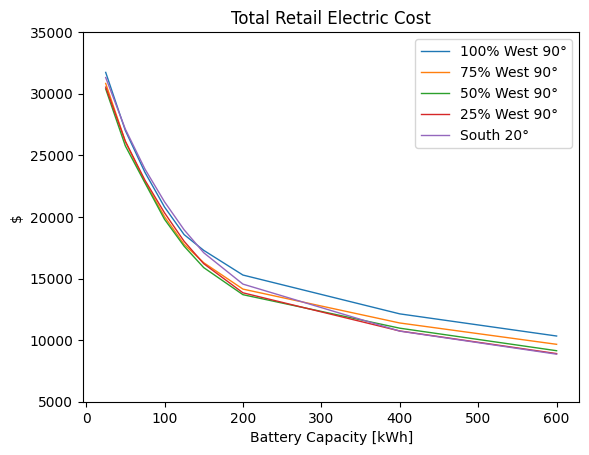
\includegraphics[width=7.5cm,height=\textheight]{./images/total cost.png}
  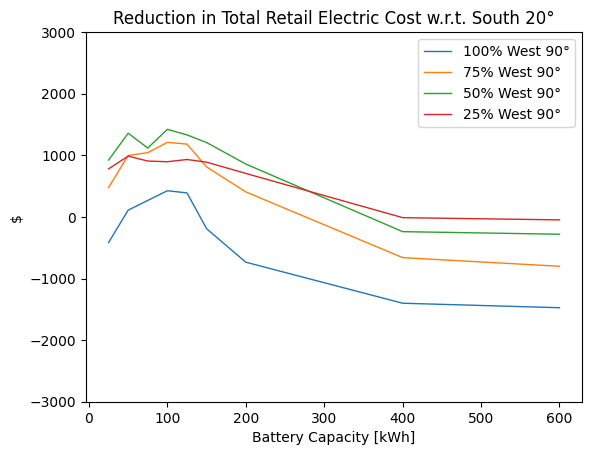
\includegraphics[width=7.5cm,height=\textheight]{./images/total cost reduction.png}
  \caption{Total Cost. Total Retail Electric Cost is calculated for each
  solar array case study and a sensitivity analysis is performed on
  battery capacity (kWh). Below 150 kW the South 20° and 100\% West 90°
  arrays have similarly high total costs, whereas the three combination
  arrays are somewhat grouped a few percent below. Above 150 kW the total
  costs for each case diverge somewhat, with the South 20° base case
  attaining the lowest cost for the 400 kWh battery and larger.
  RIGHT: Reduction in Total Retail Cost is likely the most important metric for
  evaluating the peak shaving efficacy, since it can be directly used as
  revenue in a cash flow analysis to calculate economic performance. The
  combination 50\% West 90° array with 100 kWh battery achieve the largest
  cost reduction of \$1422 (6.7\%) over the 10 month data period. A
  selection of the data generating these graphs is shown in Table \ref{tab:data-summary}.}
  \label{fig:total-cost}
\end{figure}

The benefit of vertical bifacial modules can be seen when comparing the
simulated battery charge and discharge time series data. Figure \ref{fig:peak-shaving} shows
the same day (June 6) for both the base Solar 20° case and the 100\%
West 90° case, which is presented here as a clearer graphical example
than the better performing 50\% West 90° array. For both cases June 6 is
the limiting day for the month, where the battery reaches a technical
limit, in these cases zero SOC. This is likely due to a particularly
large evening peak load event from approximately 17:30 to 21:30, with a
maximum power of 56 kW and total energy of 201 kW. For these simulations
the battery capacity is 125 kWh nominal and 112.5 kWh after losses, and
as specified the battery will charge and discharge at a maximum of 1C or
125 kW.

In Figure \ref{fig:peak-shaving} the base case of South 20° overproduces in the middle hours
of the day and solar is exported to the network starting around 12:00.
During the peak load event the South 20° only produces 18.8 kWh whereas
the 100\% West 90° array produces 104 kWh. In each case the battery
charges to 100\% (125 kWh) before the evening peak load event. The
result is that the evening net load peak in the 100\% West 90° case
starts later and contains less energy, though it reaches the same
maximum power. Due to this the battery in the 100\% West 90° case can
hold the site load to a lower threshold in \(kW\), which is directly
proportional to reducing the retail electric cost. During the expensive
"Peak" TOU period of 14:00-21:00 the base South 20° case only achieves a
low threshold of 13.0 kW, whereas the 100\% West 90° case holds a
threshold of 3.1 kW in the same period, a 76\% improvement.

The retail electric cost isn't defined for only one day out of a typical
month, since the power portion of the cost is calculated on the monthly
peak. However if June 6 was the only day of the month with non-zero load
the total cost would be \$983 for the South 20° case and \$560 for the
50\% West 90° case, which is a 43\% reduction.

\begin{figure}[!h]
  \centering
  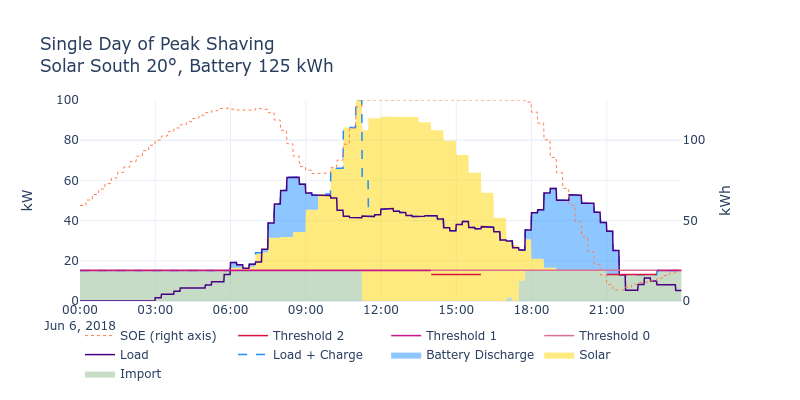
\includegraphics[width=7.5cm,height=\textheight]{./images/single day of peak shaving south.png}
  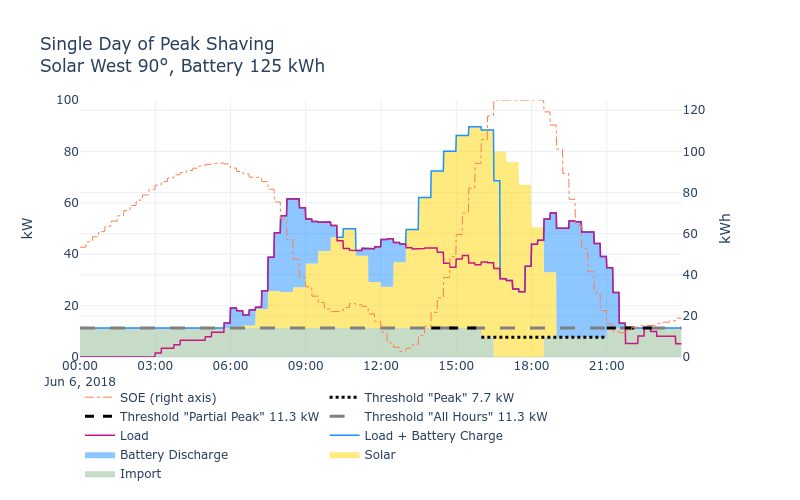
\includegraphics[width=7.5cm,height=\textheight]{./images/single day of peak shaving west.png}
  \caption{Single Day of Peak Shaving. The stacked
  dispatch plots use a convention where EV charging load (magenta) and
  stationary battery charging additional load (blue) are the solid lines,
  whereas any source of energy including the discharging battery are solid
  areas. Since load must always be equal to the sum of supplied energy,
  the areas always stack up to meet the load lines. The only exception is
  when energy is exported back to the network, as is the case with
  afternoon solar production here. The TOU power thresholds are
  represented by the four dashed line segments, which begin and end based
  on the begin and end of the TOU period, and overlap in time where the
  TOU periods overlap. SOE is the dash-dot line referenced to the right
  vertical axis. The base South 20° solar array overproduces midday
  and exports energy to the grid, leaving more energy in the evening peak
  that the stationary battery needs to serve.
  RIGHT: The 100\% West 90°
  case exports less solar to the grid, and has more late afternoon
  production aligned with the evening load peak, allowing the peak shaving
  algorithm to achieve a 42\% lower Peak period threshold of 7.7 kW than
  the South 20° array.}
  \label{fig:peak-shaving}
\end{figure}



In Table \ref{tab:total-cost} are some of the data from Figure \ref{fig:total-cost}, though not shown for
conciseness are the 75\% West 90° and the 25\% West 90° cases. The
largest cost reduction is \$1422 for the 50\% West 90° case and 100 kWh
battery. Note that the largest reduction in retail cost may not be the
best solution economically, since the 25 kWh battery achieves 65\% of
the cost reduction at 20\% of the battery energy capacity, which is
roughly proportional to capital cost.

\begin{table}[!h]
  \centering
  \caption{Total Retail Electric Cost. Simulated total
  retail electric cost for three of the case studies (some omitted for
  conciseness) over the 10 months of available data and a given battery
  capacity. Cost reduction is calculated with respect to the South 20°
  base case. The best reduction in total retail cost is \$1422 for the
  50\% West 90° case.}
  \label{tab:total-cost}
  \begin{tabularx}{\textwidth}{XXXXXXXX}
  \toprule
  Battery {[}kWh{]} & Cost South 20° {[}\${]}                & Cost 50\% West 90°
  {[}\${]}          & Cost 100\% West 90° {[}\${]}           & Cost Reduction 50\% West 90°
  {[}\${]}          & Cost Reduction 100\% West 90° {[}\${]} & Cost Reduction 50\%
  West 90° {[}\%{]} & Cost Reduction 100\% West 90°
  {[}\%{]}\\
  \midrule
  25                & 31314.0                                & 30391.0                      & 31730.0 & 923.0           & -416.0  & 3.0  & -1.3\\
  50                & 27132.0                                & 25773.0                      & 27022.0 & 1359.0          & 110.0   & 5.0  & 0.4\\
  75                & 23893.0                                & 22775.0                      & 23625.0 & 1118.0          & 268.0   & 4.7  & 1.1\\
  100               & 21229.0                                & 19807.0                      & 20804.0 & \textbf{1422.0} & 425.0   & 6.7  & 2.0\\
  125               & 18954.0                                & 17623.0                      & 18564.0 & 1331.0          & 390.0   & 7.0  & 2.1\\
  150               & 17094.0                                & 15886.0                      & 17286.0 & 1208.0          & -192.0  & 7.1  & -1.1\\
  200               & 14547.0                                & 13689.0                      & 15282.0 & 858.0           & -735.0  & 5.9  & -5.0\\
  400               & 10730.0                                & 10969.0                      & 12131.0 & -239.0          & -1401.0 & -2.2 & -13.1\\
  600               & 8859.0                                 & 9140.0                       & 10333.0 & -281.0          & -1474.0 & -3.2 & -16.6\\
  \bottomrule
  \end{tabularx}
\end{table}

A sensitivity analysis on the size of the solar array is performed with
the results in Figure \ref{fig:solar-sensitivity} and Table \ref{tab:solar-sensitivity}. The total retail cost decreases monotonically
with the larger solar capacities, and the cost reduction increases by a
factor of 10 from the smallest to largest solar capacity. This result is
expected since the larger capacities create a more pronounced difference
between the late afternoon production of the two arrays which the peak
shaving strategy translates into lower power thresholds for the cases
with some portion of the array in the 100\% West 90° orientation.

The 50\% West 90° case performs best in the first four solar capacities
at which point, for the first time, the best performing case is one
where the majority of the modules are in the 100\% West 90° orientation
(75\%). However the difference of \$19 is not substantial. At larger
solar capacities the cost reductions for each case study are both larger
in magnitude and closer together, however the increase in cost reduction
is clearly less than linear with solar capacity. This suggests a
diminishing returns problem where, after a certain capacity of 100\%
West 90° modules is met, the additional South 20° and 100\% West 90°
modules are providing energy when the battery is already at 100\% SOC.


\begin{table}[!h]
  \centering
  \caption{Solar capacity sensitivity analysis based on reduction in total
  retail cost relative to the base South 20° case. While the 50\% West 90°
  array continues to achieve the highest cost reduction, the battery
  capacity increases from 25 kWh to 125 kWh.}
  \label{tab:solar-sensitivity}
  \begin{tabularx}{\textwidth}{XXXX}
    \toprule
    Solar Capacity {[}\(kW_{DC}\){]} & Best Case for Cost Reduction         & Best
    Cost Reduction {[}\${]}          & Best Cost Reduction Battery Capacity
    {[}kWh{]}\\
    \midrule
    64.4 (0.5x)                      & 50\% West 90°                        & 260  & 25\\
    128.8 (1.0x)                     & 50\% West 90°                        & 1422 & 100\\
    193.2 (1.5x)                     & 50\% West 90°                        & 2211 & 125\\
    257.6 (2.0x)                     & 75\% West 90°                        & 2579 & 125\\
    \bottomrule
  \end{tabularx}
\end{table}


\begin{figure}
  \centering
  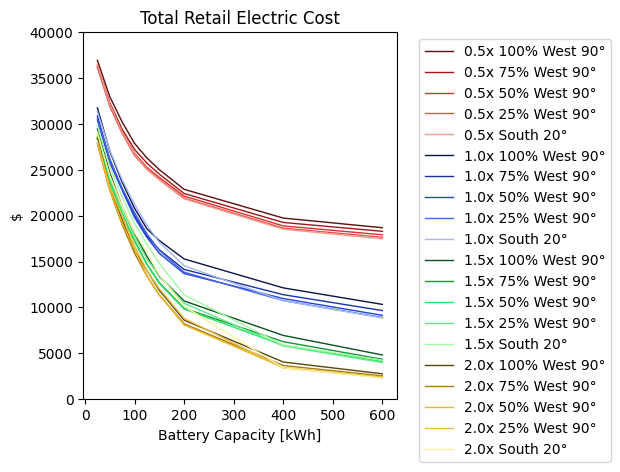
\includegraphics[width=10cm,height=\textheight]{./images/total cost reduction solar sensitivity.png}
  \caption{Solar Capacity Sensitivity. A sensitivity
  analysis on solar capacity shows more available cost reduction, which
  increases less than linearly with solar capacity.}
  \label{fig:solar-sensitivity}
\end{figure}

The battery capacities increase from 25 kWh up to 125 kWh across the
solar sizes, which is an unexpected finding. Despite the extra capacity
the 100\% West 90° case in Figure \ref{fig:weekly-load-solar} is still mostly unable to affect the
peak power of the evening peaks, and thus both the base South 20° and
combination array cases have a similar maximum power to shave. Indeed
the average of the monthly peak net load values is 74.5 kW for the South
20° 2.0x case and 74.7 kW for the 100\% West 90° 2.0x case. However,
when increasing the solar to 2.0x, the energy under the net load time
series during the 17:00 to 22:00 period decreases by only 164 kWh for
the South 20° versus 886 kWh for the 100\% West 90° case. With more
solar production in the evening peak the optimizer is able to pursue
driving the "Peak" TOU period to zero, which has a large economic
benefit. This is unachievable with the small battery capacities and is
more difficult without the late afternoon solar production of the 100\%
West 90° modules. Indeed a large 200 kWh battery is required to achieve
the first 0 kW "Peak" period threshold in the South 20° case for all
solar capacities. Rather, the 100\% West 90° case achieves a 0 kW Peak
period threshold with the 150 kWh battery at 100\% solar capacity and
with the 125 kWh battery at 2.0x solar capacity.

\begin{figure}
  \centering
  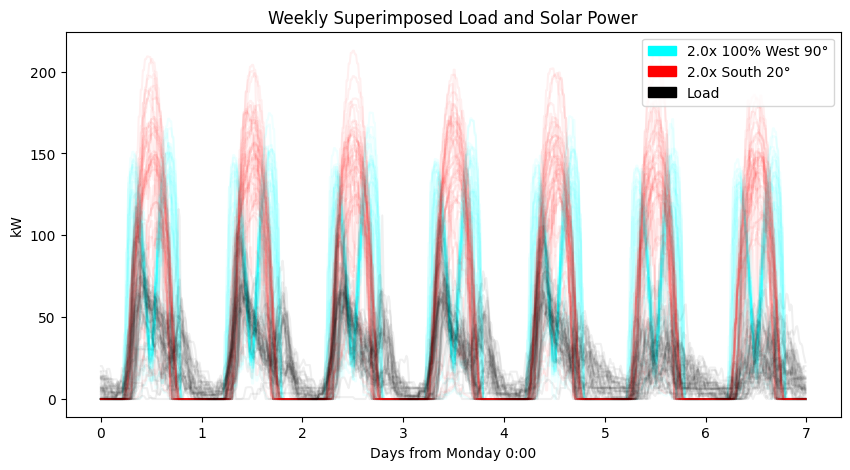
\includegraphics{/home/mjw/Code/Bifacial-solar-and-peakshaving/Paper/images/bifacial_peak_shaving_paper.assets/weekly load solar.png}
  \caption{Weekly Overlaid Load and Solar Power. The
  entire 10 month time series of EV charging load, Solar 20°, and 100\%
  West 90° are superimposed on a weekly basis, beginning on Monday. The
  100\% West 90° case provides a clearer graphical example than the better
  performing cases.}
  \label{fig:weekly-load-solar}
\end{figure}

\hypertarget{conclusion}{%
  \section{Conclusion}\label{conclusion}}

An optimal electric load peak shaving strategy is simulated on 10 months
of EV charging power time series. The peak shaving asset is a storage
battery with a maximum charge and discharge rate of 1C and a constant
discharge and charge efficiency of 90\%. A co-located solar array is
included in the simulation to study the effects of typical South facing
modules vs West facing vertical bifacial modules. Five different array
orientations are presented as different case studies. In addition
sensitivity analyses on battery energy capacity and solar array capacity
provide information about the dynamics of the optimal peak shaving
algorithm. The best performing case is designed with 50\% of the array
South facing tilted at 20° and 50\% facing West at 90°, which achieved a
reduction in the total retail cost of energy of \$1422 (6.7\%) with a 25
kWh battery. The cost reduction is relative to the base case array with
all the modules facing South and tilted at 20°. When solar is increased
to twice the net-zero capacity the best performing case is 75\% West 90°
with a cost reduction of \$2579 (16.1\%) with a 125 kWh battery. The
best percentage cost reduction overall is 20.0\%. Both data and code are
shared to the public on GitHub.

Peak shaving a monthly peak power typically, depending on the load
factor, results in dispatching the battery until its technical limits to
achieve a minimum monthly peak power. Because the load, or net load
after solar is dispatched, is often not very homogeneous there will be
one limiting day where the battery is bound by its technical limits and
the peak power of the month is set. The presence of this limiting day in
the month simulation of Figure \ref{fig:peak-shaving} does not guarantee a global minimum
cost, but the lack of a limiting day would suggest the global minimum
was not found. Intuitively the limiting day can be thought of as the
most difficult day for the battery to achieve the given thresholds, and
if the day was somehow easier for the battery (less and more uniform net
load) the power thresholds could be lowered and therefore a lower retail
electric cost achieved. Because the results of each month typically
depend strongly on one limiting day, small changes in the load or solar
magnitude or temporal relationship can have a large impact on the
overall results. For this reason peak shaving simulations require
particular care into data selection, cleaning, and acquiring an
appropriate large amount of data such that the probability space of true
possible limiting is well represented in the selected sample of limiting
days.

Confidence in the results presented is medium-high given the use of true
EV charging measurements, a robust Newton-Raphson gradient descent
optimizer with verified optimality, a true electric tariff appropriate
for the load site and solar data location, and sensitivity analyses
performed on two variables. Future work should include a more load data
sets with more months of data, a more comprehensive battery model, an
operational version of the peak shaving strategy, and testing at the
Politecnico di Milano M2GLab microgrid.

\hypertarget{bibliography}{%
  \section{Bibliography}\label{bibliography}}

\end{document}
